\subsection{Jets}
\label{sec:jet}

Jets are another important features for many physics analyses at the LHC, and especially the key signatures for vector boson fusion/scattering (VBF/VBS) processes.
In ATLAS detector, jets are reconstructed as groups of topologically associated energy deposits in the calorimeters, 
tracks associated with charged particles measured in the inner tacking detector, or simulated particles.
This section introduces the jet reconstruction, jet energy scale (JES) calibration and the b-jet tagging technical.

\textbf{Jet reconstruction}

Jets are reconstructed using anti-$k_{t}$ algorithm\cite{Cacciari_2008} and with radius parameter of $R = 0.4$ in most cases.
The \textsc{FastJet} software package\cite{Cacciari2012} is utilized for jet finding and reconstruction.
A collection of four-vectors are used as inputs at each combination step in jet clustering, 
the total four-momentum is therefore computed as the sum of four-vector of all its constituents.
There are three types of jets in ATLAS:
\begin{itemize}
	\item \textit{Truth jets:} the inputs to jet algorithm are simulated particles.
	\item \textit{Track jets:} the inputs are charged tracks measured from inner detector.
	\item \textit{Calorimeter jets:} the inputs are energy deposits in calorimeters.
\end{itemize}
Figure~\ref{fig:jet_reco_overview} shows the schematic of ATLAS jet reconstruction.
\begin{figure}[!htb]
  \centering
  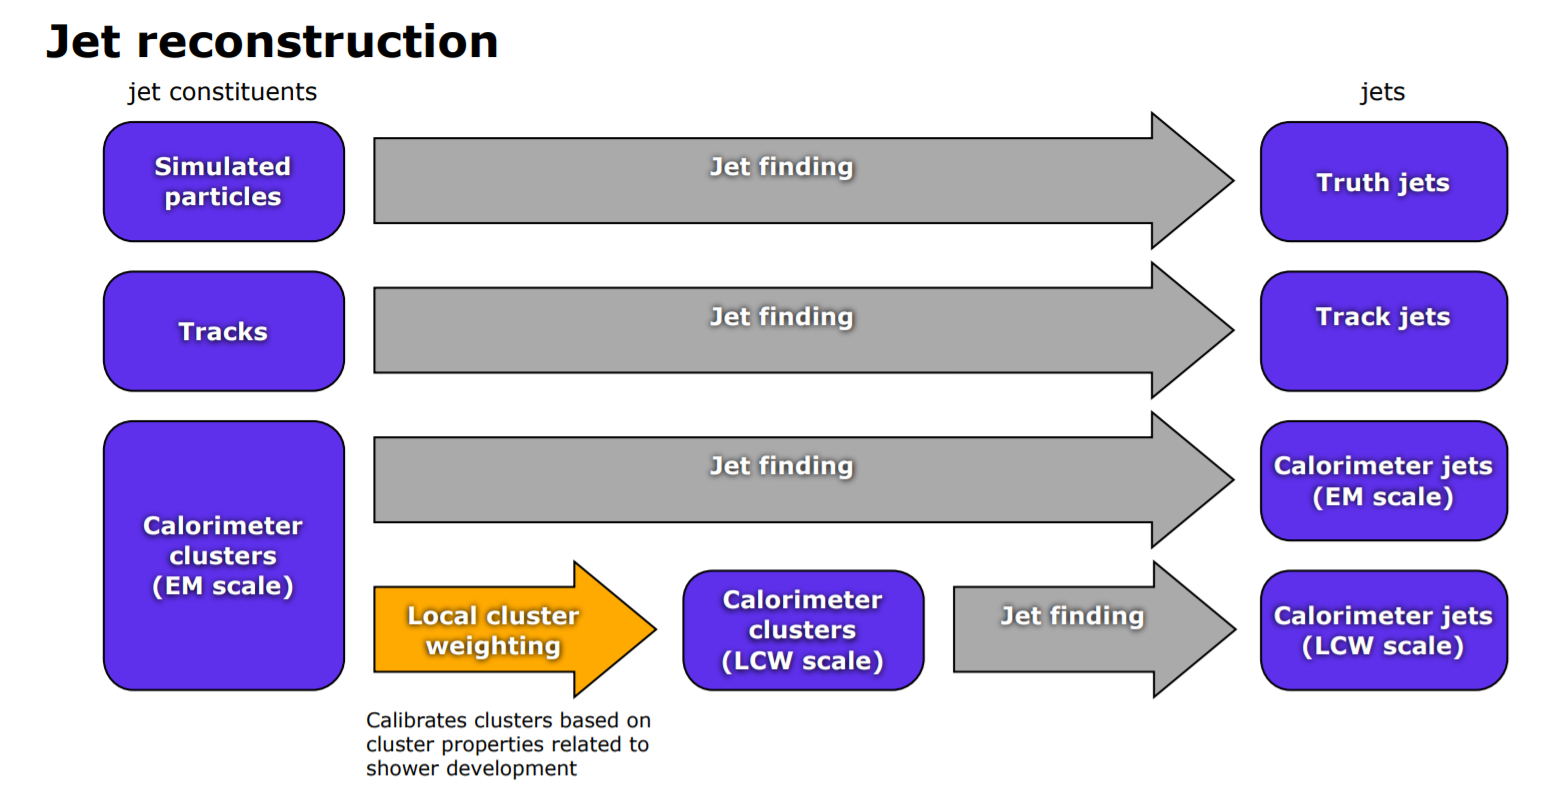
\includegraphics[width=1.0\textwidth]{figures/Simulation/threetypes_jet_reco.png}
  \caption{A overview schematic of ATLAS jet reconstruction\cite{Aad:2014bia}.}
  \label{fig:jet_reco_overview}
\end{figure}

The \textit{truth jets} are reconstructed using anti-$k_{t}$ algorithm with $R = 0.4$ by using final-state, stable particles from MC simulation as inputs.
It requires the candidate particles with lifetime $c_{\tau}$ > 10 mm and excludes the particles from pile-up.
Truth jets with $p_{T} > 7 GeV$ and $|\eta| < 4.5$ are then used for jets calibration described later.

The \textit{track jets} are reconstructed from charged particles within the full acceptance of inner detector ($|\eta| < 2.5$).
The track reconstruction has been introduced in section~\ref{sec:track}.
Reconstructed jets with $p_{T} > 500 MeV$ and associated with primary vertex are then selected.
Tracks are assigned to jets using ghost association\cite{CACCIARI2008119}, a procedure that treats selected tracks as four-vectors of infinitesimal magnitude during the jet reconstruction and assigns them to the jet which they are clustered with.
In addition, muon track segments are used as a compensation for those uncaptured jet energy carried by energetic particles passing through the calorimeters without being completely absorbed.
Similar to the ID track, muon segments are assigned to jets using the method of ghost association mentioned above as well.

The \textit{calorimeter jets} are reconstructed using a set of three-dimensional, positive-energy topological clusters (topo-clusters) made of calorimeter cell energies as input to the anti-$k_{t}$ algorithm\cite{Aaboud:2017jcu}.
Topo-clusters are built from near-by calorimeter cells that contains a significant energy above a noise threshold,
which is estimated from measurements of calorimeter electronic noise and simulated pile-up noise.
Those calorimeter cell energies are measured at electromagnetic energy scale (EM scale) corresponding to the energy deposited by electromagnetically interacting particles. 
And jets passing a \pt threshold of 7 GeV are reconstructed with the anti-$k_{t}$ algorithm.

\textbf{Jet energy scale calibration}

Figure~\ref{fig:jet_cali} depicts an overview of ATLAS jet calibration scheme for EM-scale calorimeter jets.
In this procedure, the jet energies are scaled to truth jets, which is reconstructed at the particle-level.
Each step of the calibration corrects the full four-momentum unless otherwise stated, scaling the jet \pt, energy, and mass.
\begin{figure}[!htb]
  \centering
  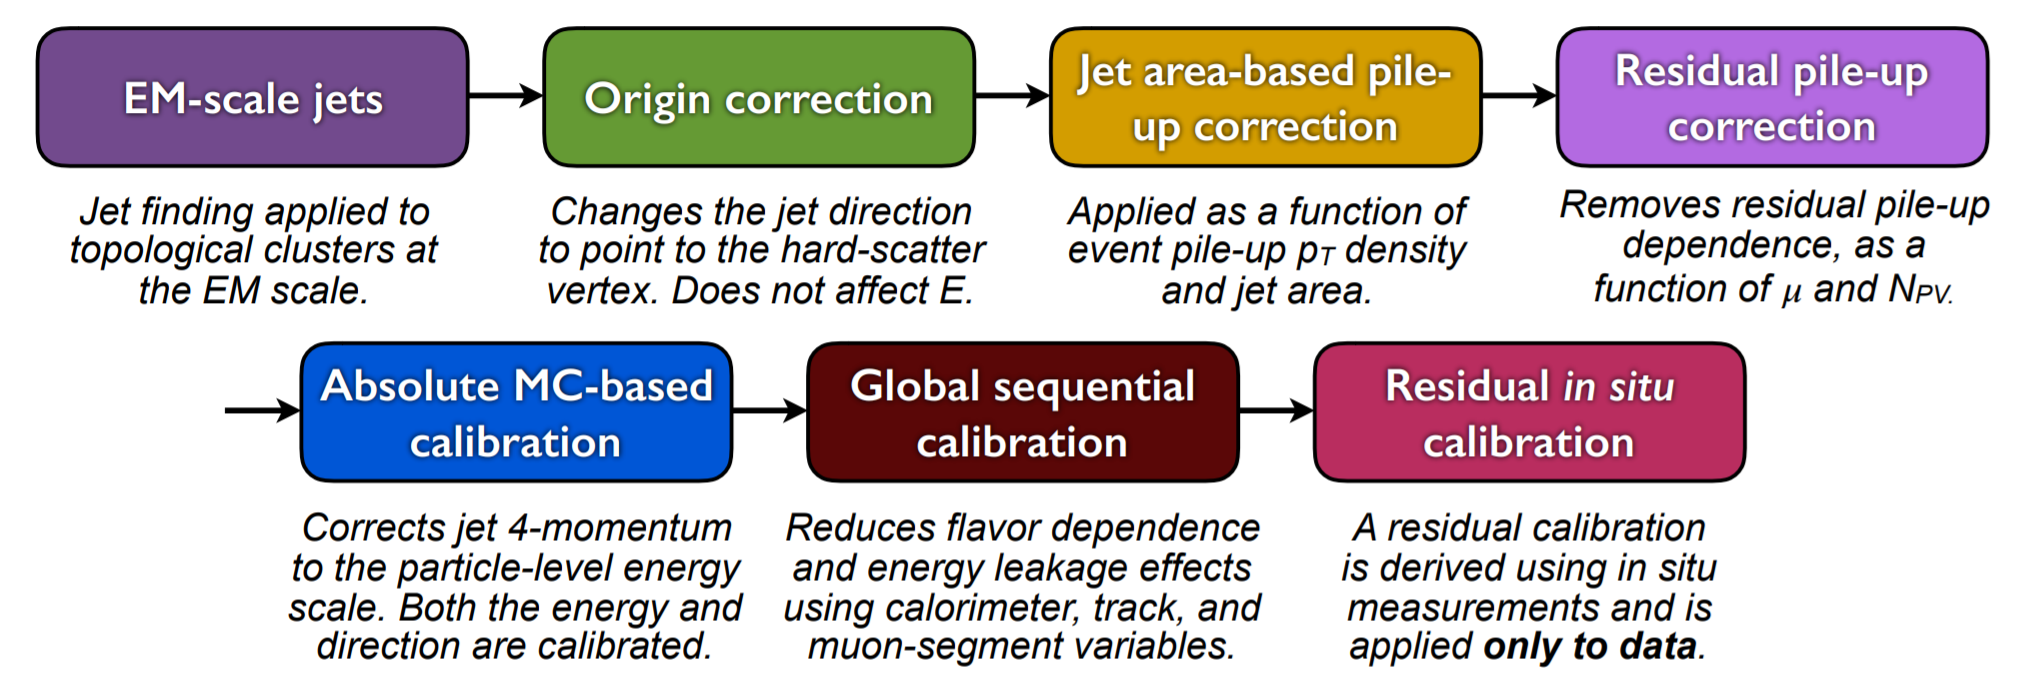
\includegraphics[width=1.0\textwidth]{figures/Simulation/jet_calibration.png}
  \caption{A overview schematic of ATLAS jet calibration\cite{Aaboud:2017jcu}.}
  \label{fig:jet_cali}
\end{figure}

First of all, the origin correction recompute the four-momentum of jets to point them to the hard-scatter primary vertex instead of the centre of detector, and in the meantime keep the jet energy unchanged.
This correction improves the $\eta$ resolution of jets for roughly 25\% at a jet $p_{T}$ of 20~\gev~ and > 5 times improvement for jet with $p_{T}$ above 200~\gev, 
as measured from the difference between reconstructed jets and truth jets in MC simulation.
Secondly, the pile-up correction is adopted to remove the excess energy due to in-time and out-of-time pile-up,
which consists of two processes: an area-based $p_{T}$ density subtraction applied on the top of each event; and a residual correction derived from the simulation.
Thirdly, the absolute JES calibration corrects the jet four-momentum to the particle-level energy scale, using truth jets in di-jet MC events.
Furthermore, the step of global sequential calibration uses calorimeter, track and MS-based variables to reduce the flavor dependence and energy leakage effects.
Finally, the residual in situ calibration is adopted to correct jets in data by using well-measured objects eg. photons, Z bosons and calibrated jets.

\textbf{B-jet tagging}

Tagging of b-jets plays a important role in many physics analyses involving b- or t- quark.
In the meantime, lots of analyses need to apply b-jet veto to suppress \ttbar process.
There are three major types of algorithms that have been developed to distinguish b-quark jets from light-quark (u,d,s) jets~\cite{ATL-PHYS-PUB-2016-012}:
\begin{itemize}
	\item \textbf{Impact parameter based algorithms (IP2D and IP3D):} b-hadrons usually have long lifetime ($\sim$1.5 ps, $c_{\tau}\sim450~\mu$m), which leads to large impact parameter for tracks produced from b-hadron decay. The impact parameter taggers are developed based on these variables. The IP2D tagger makes use of the transverse impact parameter significance $d_{0}/\sigma(d_{0})$ as discriminant, while IP3D tagger uses two-dimensional discriminant of both transverse and longitudinal impact parameter significances: $d_{0}/\sigma(d_{0})$ and $z_{0}sin\theta/\sigma(z_{0})$.
	\item \textbf{Secondary vertex finding algorithm (SV1)} makes use of the secondary vertex formed by decay products of b-hadron within the jet. All track pairs within a jet are tested for a two-track vertex hypothesis, and removed if they are likely to originate from a long-live particle decay (eg. $K_{s}$ or $\Lambda$), hadronic interactions or photon conversions. After that, a new vertex is fitted with all tracks from remaining two-track vertices, and the outliers are removed from this set of tracks.
	\item \textbf{Decay chain multi-vertex algorithm (JetFitter)}\cite{Piacquadio_2008} exploits the topological structure of weak b- and c- hadron decays inside the jet and tries to reconstruct the full b-hadron decay chain. A Kalman filter is adopted to find a common line between primary vertex and b-/c- vertices, as well as their position in this line, which gives a approximated flight path for the b-hadron. In this approach, the b- and c-hadron vertices, whenever resolution allows, can be resolved, even when there is only a single track associated to them.
\end{itemize}
The final discrimination commonly used in many physics analyses is called \textbf{Multivariate Algorithm (MV2)}, which is based on Boosted Decision Tree (BDT) implemented in the TMVA package\cite{Speckmayer_2010} by combining the outputs from underlaying taggers mentioned above.
The MV2 was trained using jets in $t\bar{t}$ sample, where the b-jets are treated as signal while the c- and light-flavor jets are treated as backgrounds.
There are three kinds of MV2 depending on the fraction of c-jets in background for training: \textit{MV2c00}, \textit{MV2c10} and \textit{MV2c20}.
Figure~\ref{fig:jet_mv2} presents the output score of MV2c10 for different flavor jets.
\begin{figure}[!htb]
  \centering
  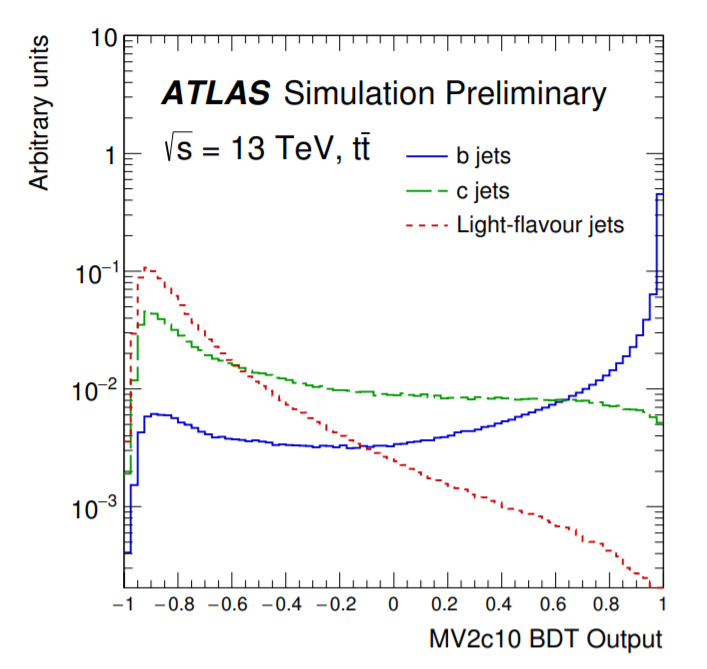
\includegraphics[width=0.5\textwidth]{figures/Simulation/jet_mv2c10.png}
  \caption{MV2c10 BDT output for b- (solid blue), c- (dashed green) and light-flavour (dotted red) jets in $t\bar{t}$ events\cite{ATL-PHYS-PUB-2016-012}.}
  \label{fig:jet_mv2}
\end{figure}
